\chapter{Curve fitting of potential for MMO without photoemission}
\label{sec:second-app}
\newenvironment{longlisting}{\captionsetup{type=listing}}{}

\begin{center}
\begin{figure}[H]
  \begin{subfigure}[b]{0.61\textwidth}
    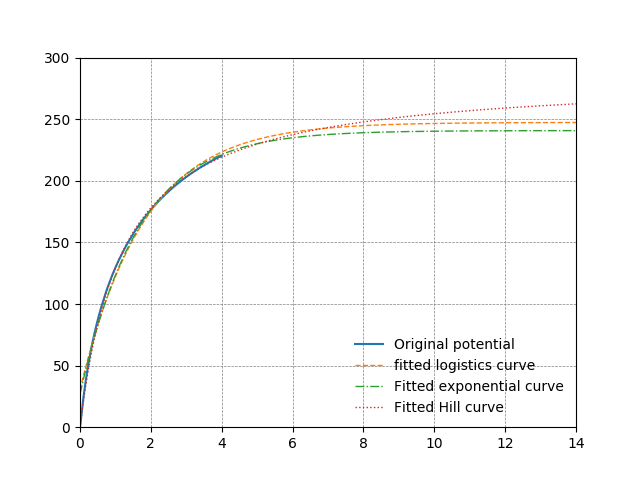
\includegraphics[width=\textwidth]{figures/Appendix/C_fit_NB.png}
    \caption{14,000 timesteps}
    \label{fig:C_fit_NB}
  \end{subfigure}
  \hfill
  \begin{subfigure}[b]{0.61\textwidth}
    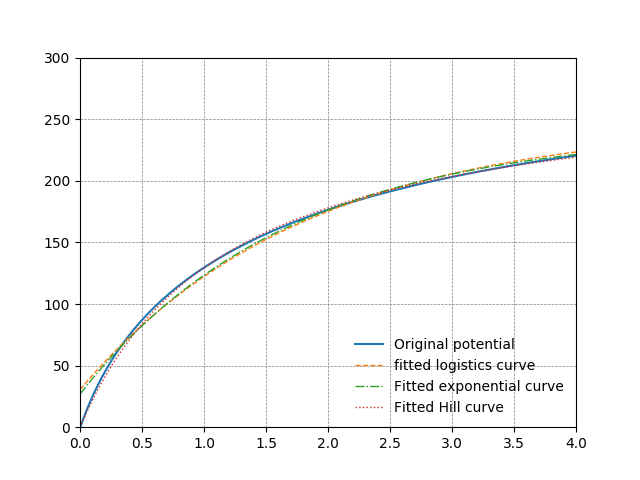
\includegraphics[width=\textwidth]{figures/Appendix/C_fit_NB_lim.png}
    \caption{4,000 timesteps}
    \label{fig:C_fit_NB_lim}
  \end{subfigure}
  \label{fig:Pot_noPH}
  \caption{Curve fitting using a generalized logistic function, Hall function, and exponential function of the potential of the MMO spacecraft without booms}
\end{figure}
\end{center}

\begin{center}
\begin{figure}[H]
  \begin{subfigure}[b]{0.61\textwidth}
    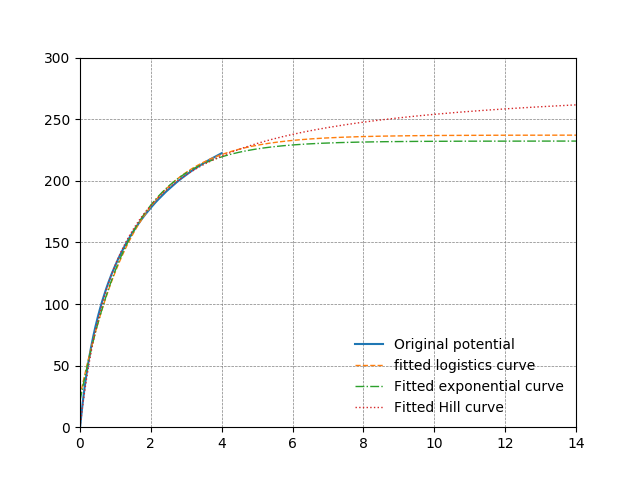
\includegraphics[width=\textwidth]{figures/Appendix/C_fit_WB.png}
    \caption{14,000 timesteps}
    \label{fig:C_fit_NB}
  \end{subfigure}
  \hfill
  \begin{subfigure}[b]{0.61\textwidth}
    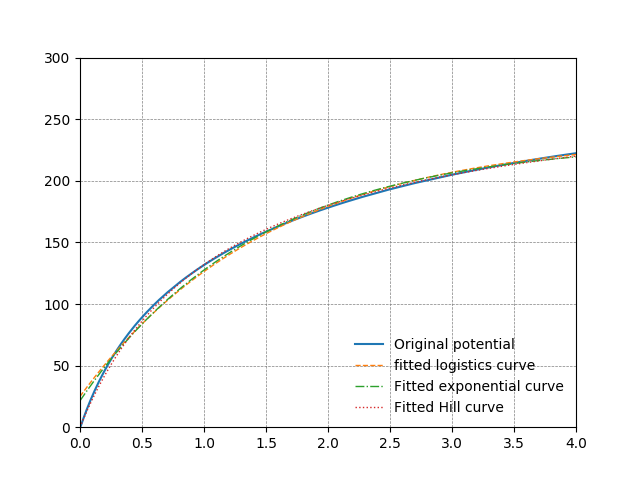
\includegraphics[width=\textwidth]{figures/Appendix/C_fit_WB_lim.png}
    \caption{4,000 timesteps}
    \label{fig:C_fit_NB_lim}
  \end{subfigure}
  \label{fig:Pot_noPH}
  \caption{Curve fitting using a generalized logistic function, Hall function, and exponential function of the potential of the MMO spacecraft with booms}
\end{figure}
\end{center}


\begin{longlisting}
\inputminted[
frame=lines,
framesep=2mm,
fontsize=\small
]{Python}{noPH_polyfit.py}
\caption{Dummy text}
\label{lst:polyfit}
\end{longlisting}